\section{Baterías de ion-litio}

Premdio Nobel...

\begin{figure}[h!]
    \centering
    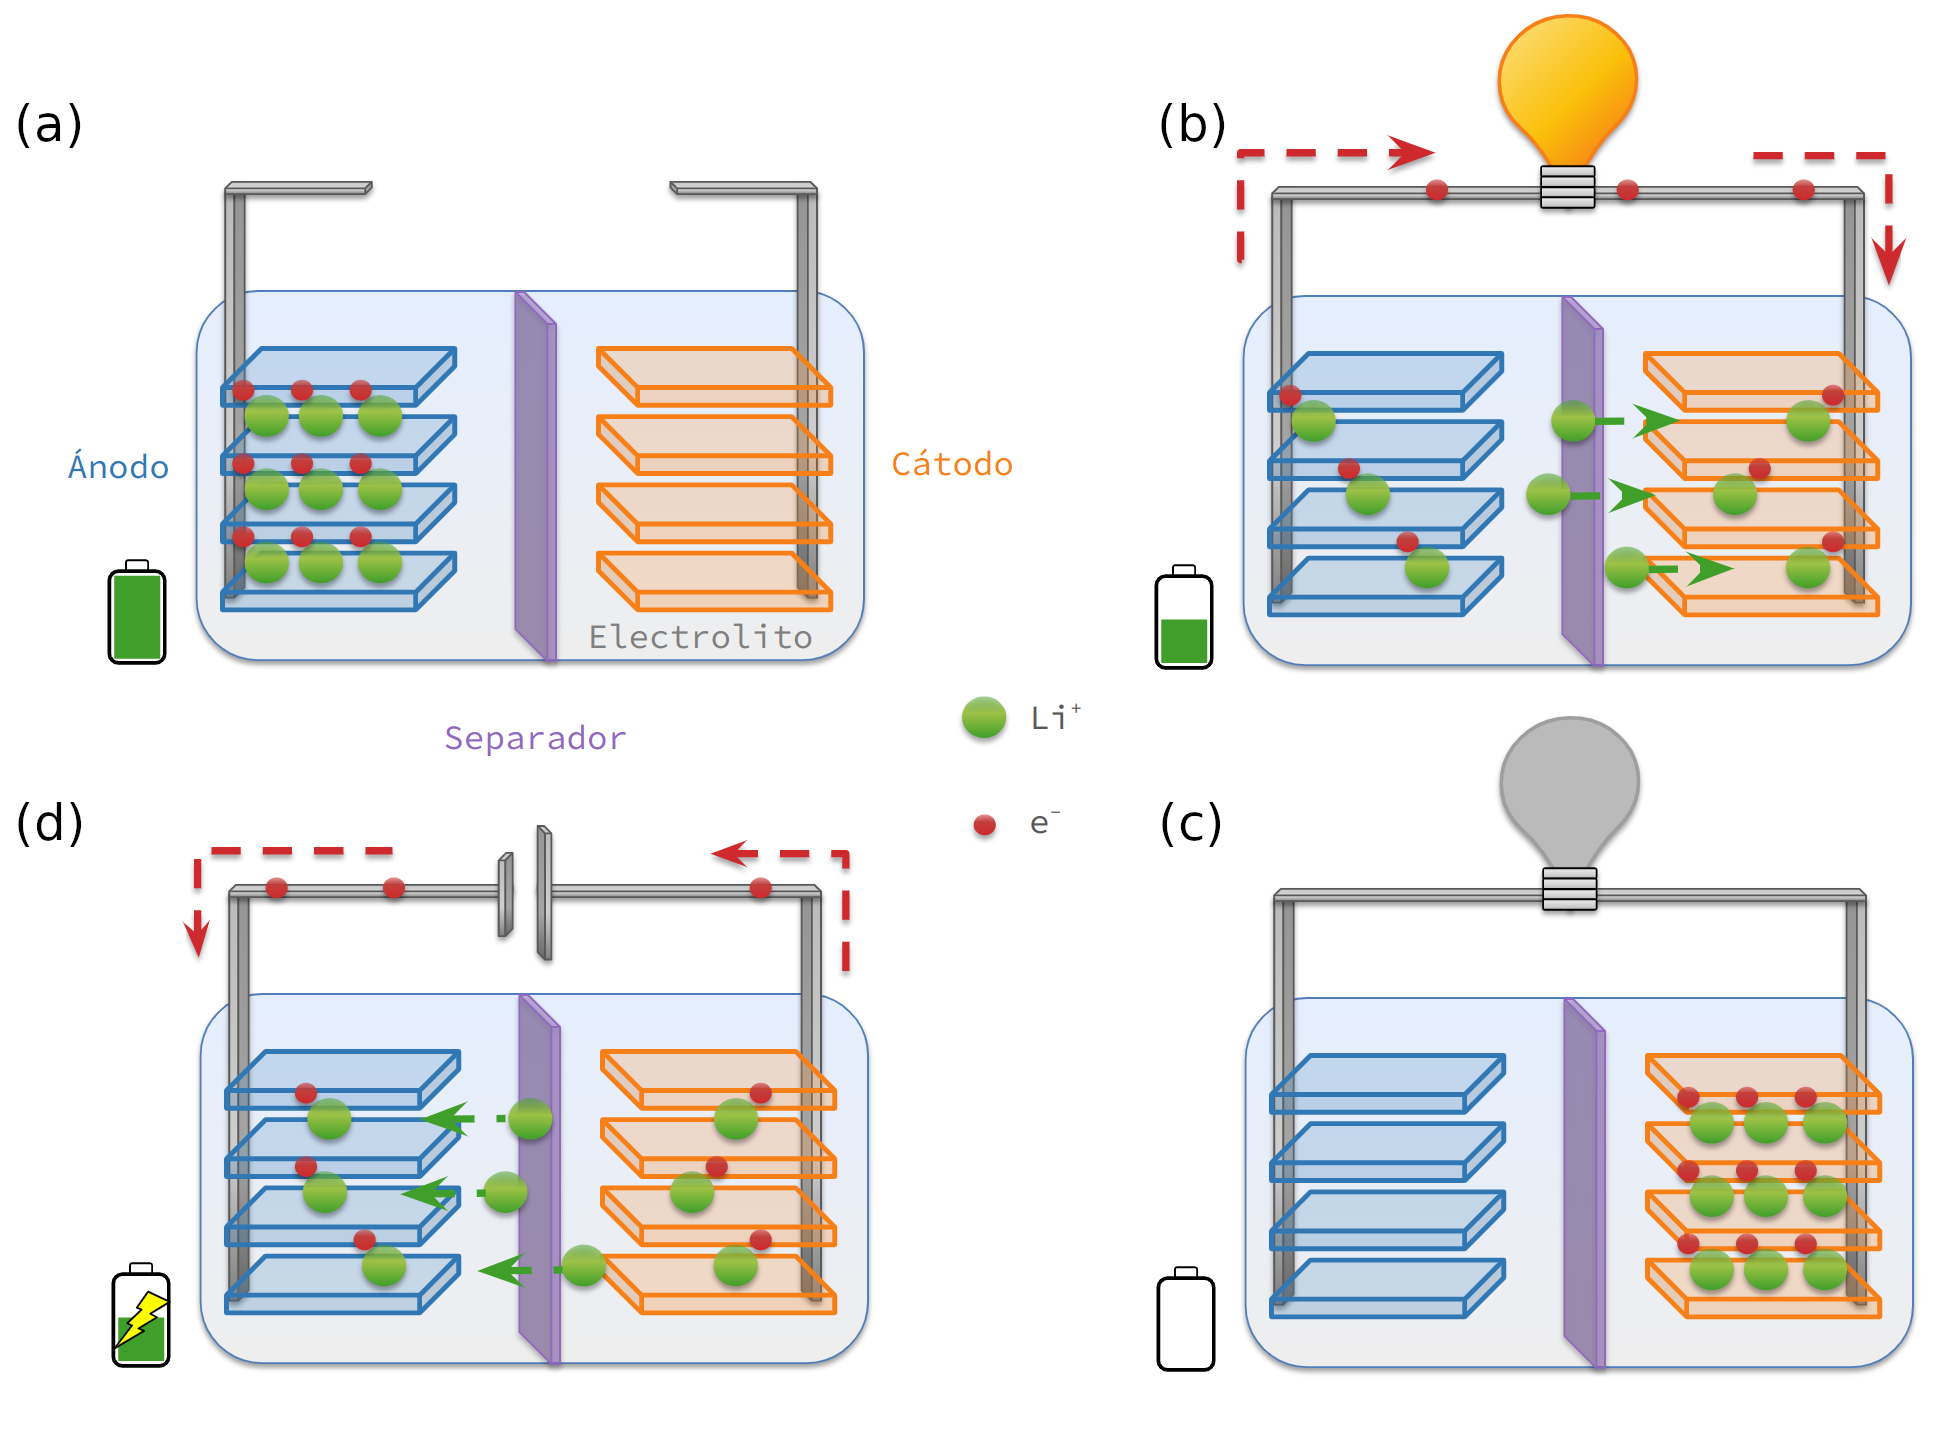
\includegraphics[width=.8\textwidth]{Introduccion/baterias/esquema_bateria.png}
    \caption{Esquema de las componentes y el funcionamiento de una batería de 
    ion-litio.}
    \label{fig:esquema-bateria}
\end{figure}

En la Figura \ref{fig:scopus} se muestra el incremento en las últimas dos décadas
de los artículos científicos publicados en el área de las baterías de litio y, en 
particular, de las dos ramas estudiadas en esta tesis: la Carga rápida y los 
Ánodos de Si. En dicha figura se presentan datos extraídos de la base de datos 
Scopus \cite{SCOPUS} del número de publicaciones anuales normalizado con respecto 
al número de publicaciones en el año 2003, año en el que hubo 710 publicaciones 
en baterías de litio, 32 sobre ánodos de Si y 0 sobre carga rápida, por lo que 
se normalizó en este caso a la única publicación del 2004 en el tema.
\begin{figure}[h!]
    \centering
    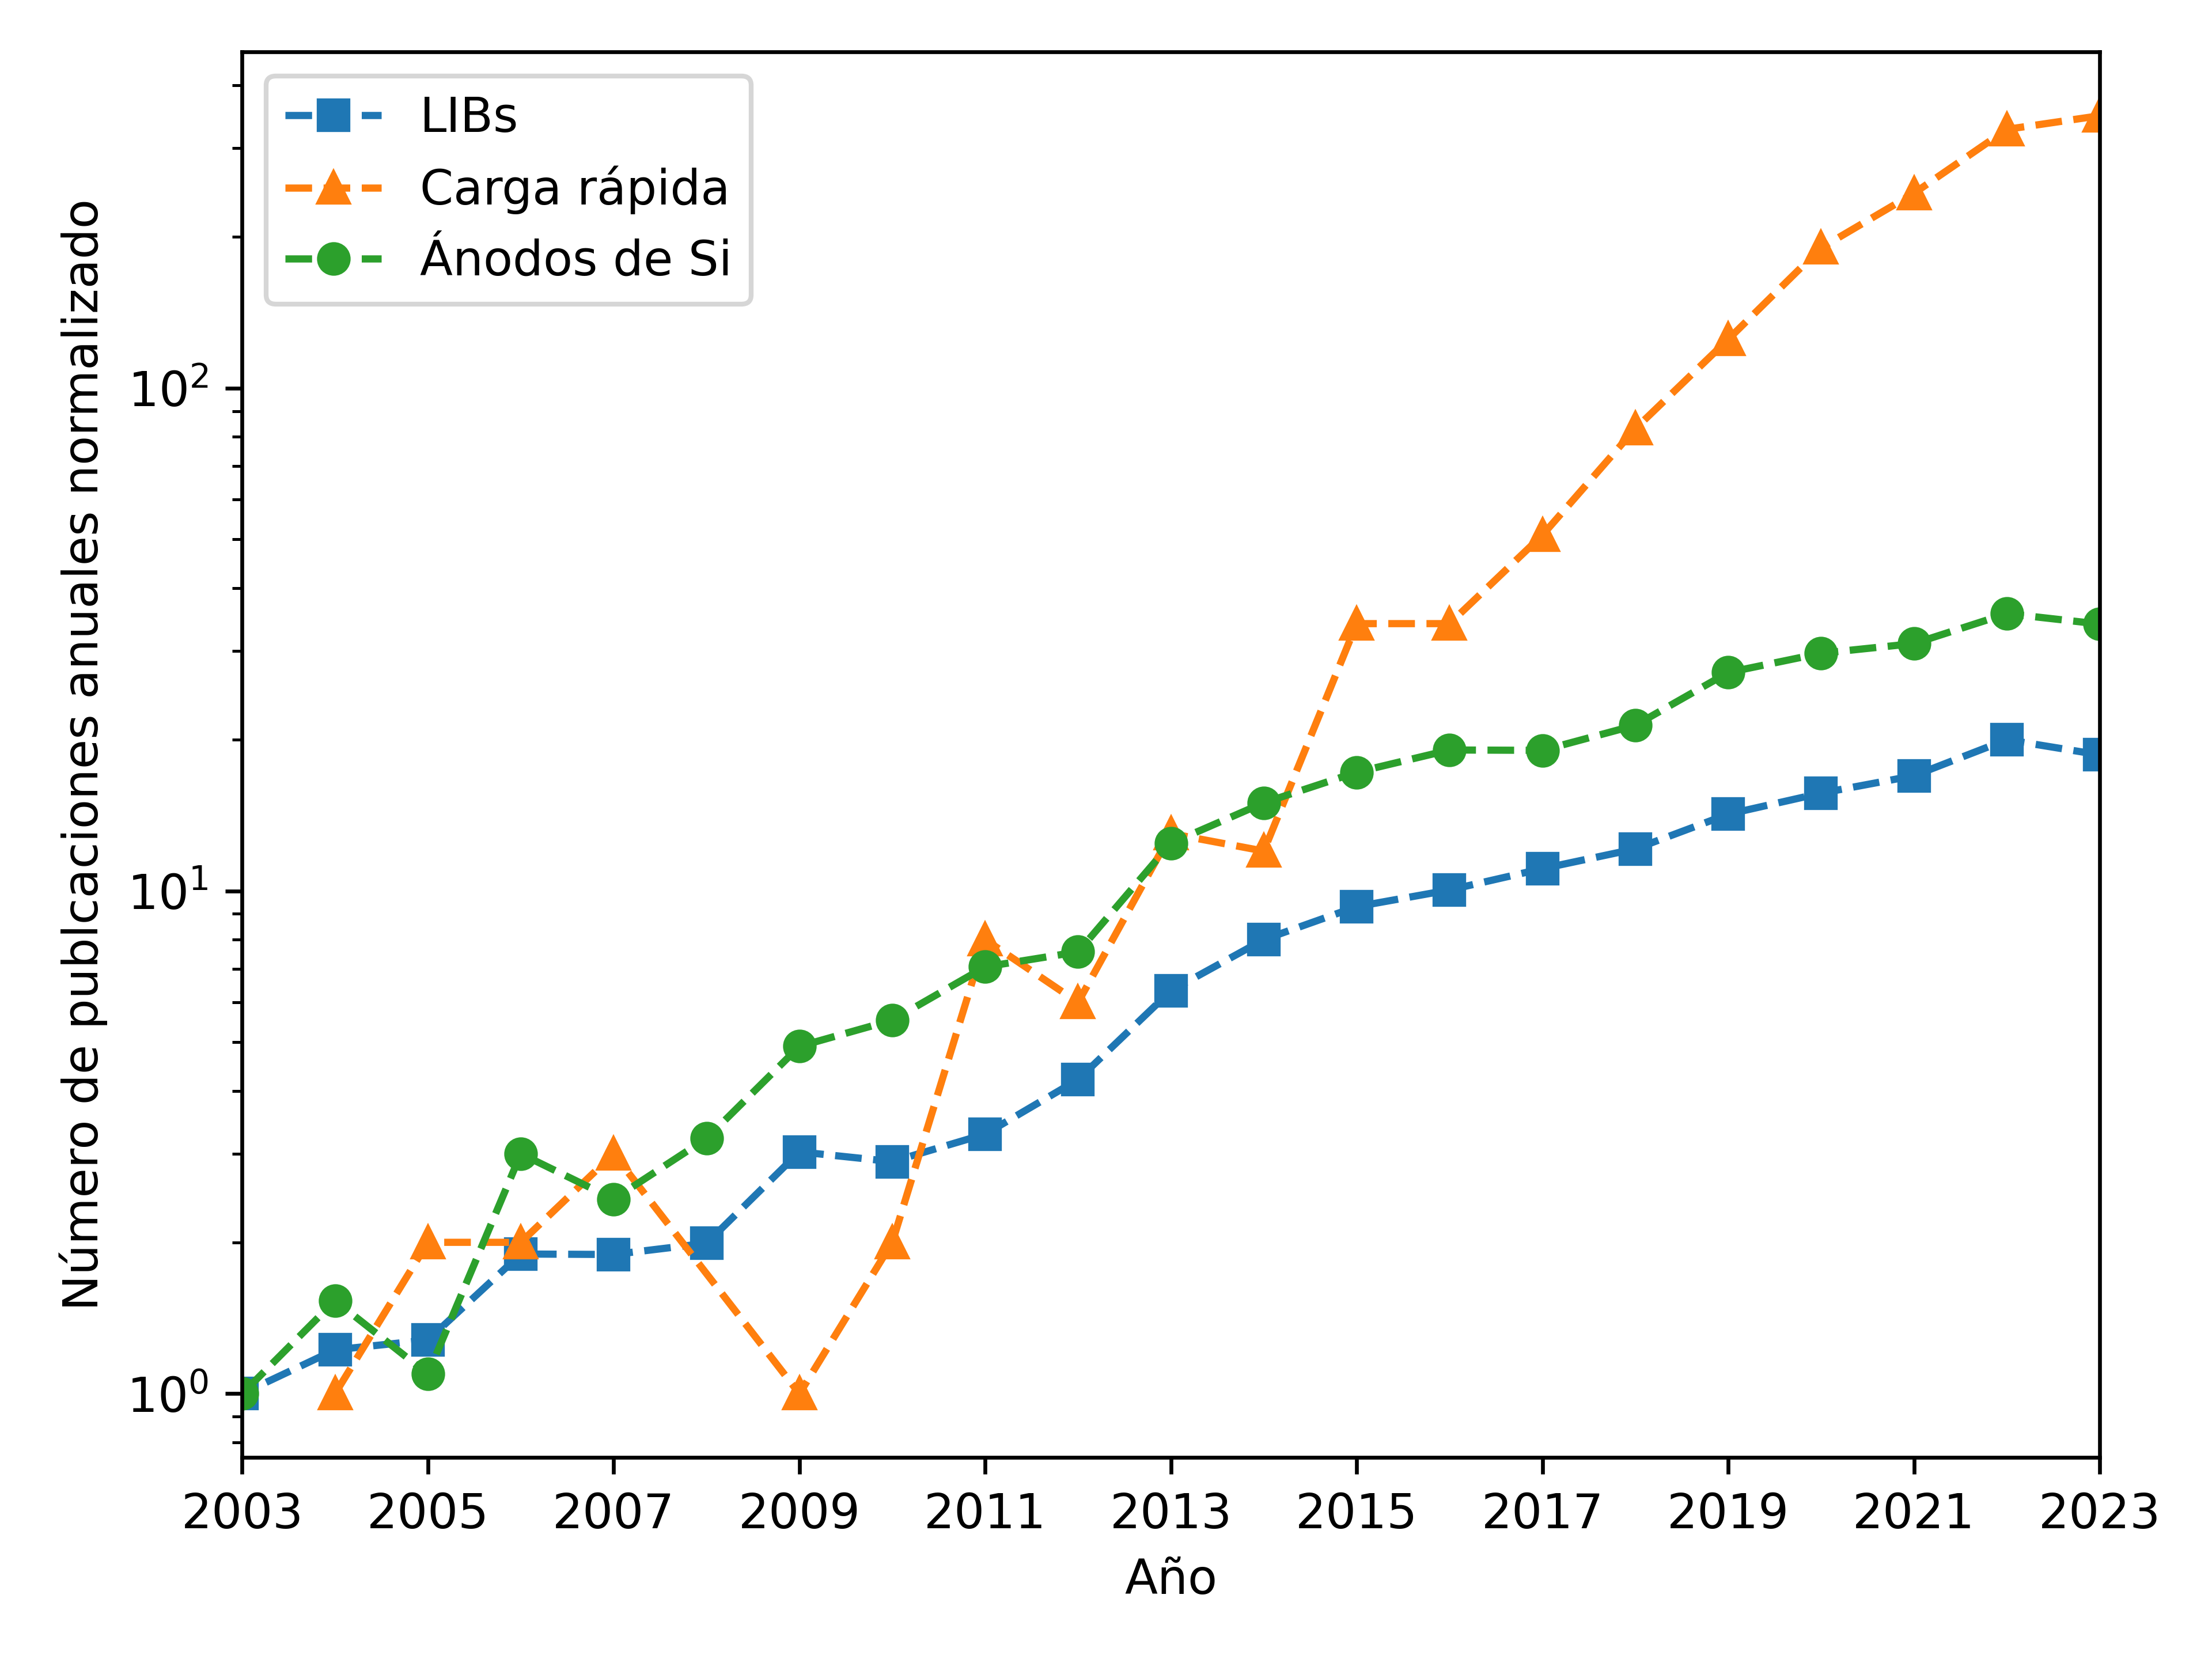
\includegraphics[width=.8\textwidth]{Introduccion/baterias/scopus.png}
    \caption{Número de publicaciones anuales normalizado con respecto al año 2003. 
    Las consultas realizadas en Scopus \cite{SCOPUS} incluyen: 
    \texttt{lithium AND battery} (LIBs, en azul), \texttt{lithium AND battery AND 
    fast-charging} (Carga rápida, en naranja) y \texttt{lithium AND battery AND 
    silicon anodes} (Ánodos de Si, en verde).}
    \label{fig:scopus}
\end{figure}
La normalización y la escala logarítmica en la Figura \ref{fig:scopus} permiten
observar cualitativamente que la pendiente de crecimiento de publicaciones 
realcionadas a la carga rápida de baterías de litio es considerablemente mayor a 
de las otras dos. Además, los ánodos de Si se encuentran dentro de lo que sería
el creciemiento promedio del área de las baterías de litio. Un análisis de datos
cuantitativo permite determinar que en la última década el aumento de porcentaje
anual de publicaciones promedio fue del 15 \% y 16 \% para las baterías de litio 
y para los ánodos de silicio, respectivamente, mientras que para la carga rápida 
este porcentaje promedio asciende al 52 \%. Este análisis demuestra la relevancia
que la comunidad científica le da a los temas estudiados en esta tesis.
